
\documentclass[11pt, a4paper]{article}

\usepackage[english, greek]{babel}
\usepackage{graphicx}
\usepackage{geometry}
\usepackage{float}
\usepackage{hyperref}
\usepackage{amsmath} % Added for equation environments
\usepackage{tikz}
\usetikzlibrary{shapes.geometric, arrows, positioning}

\geometry{a4paper, margin=1in}
\hypersetup{colorlinks=true, linkcolor=blue, urlcolor=blue, citecolor=blue}

\title{Methodology for Selecting the Experimental Area}
\author{Generated by Gemini AI}
\date{\today}

\begin{document}
\selectlanguage{english}

\maketitle

\section{Introduction}
This document outlines a methodology for selecting a specific geographic subset of data from a larger collection of points. The core of the process is to define a rectangular area of interest and then programmatically filter the dataset to retain only the points that fall within this area's boundaries. This selection process is automated to ensure precision and repeatability, with the final subset of data being saved for further analysis. A separate process is used to generate visualizations of the selected area.

\section{Process Description}

The filtering process begins by loading a dataset of geographic coordinates from a source file (e.g., a CSV or Excel file). The core logic for selecting the desired subset of data is described in the following flowchart:

\begin{figure}[H]
    \centering
    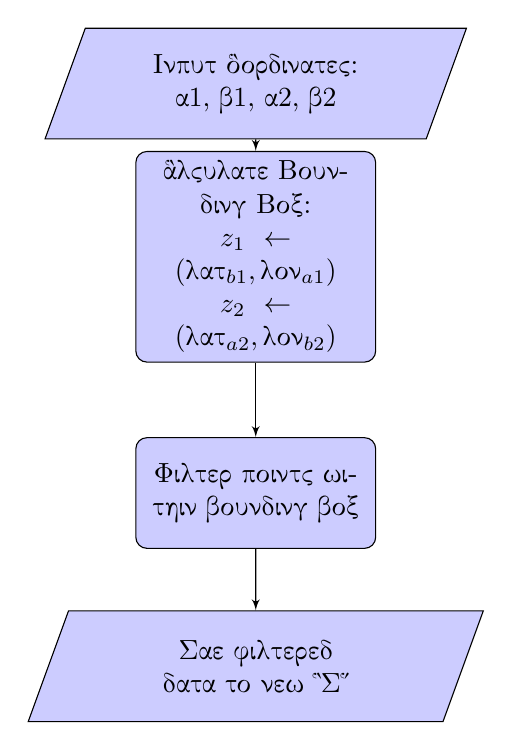
\begin{tikzpicture}[node distance=2.2cm, auto]
        \tikzstyle{block} = [rectangle, draw, fill=blue!20, 
            text width=8em, text centered, rounded corners, minimum height=4em]
        \tikzstyle{line} = [draw, -latex']
        \tikzstyle{io} = [trapezium, trapezium left angle=70, trapezium right angle=110, draw, fill=blue!20, text width=8em, text centered, minimum height=4em]

        \node [io] (input) {Input Coordinates: a1, b1, a2, b2};
        \node [block, below of=input] (calculate) {Calculate Bounding Box: \\ $z_1 \leftarrow (\text{lat}_{b1}, \text{lon}_{a1})$ \\ $z_2 \leftarrow (\text{lat}_{a2}, \text{lon}_{b2})$};
        \node [block, below of=calculate, node distance=3cm] (filter) {Filter points within bounding box};
        \node [io, below of=filter] (output) {Save filtered data to new CSV};

        \path [line] (input) -- (calculate);
        \path [line] (calculate) -- (filter);
        \path [line] (filter) -- (output);
    \end{tikzpicture}
    \caption{Flowchart of the area selection logic.}
    \label{fig:flowchart}
\end{figure}

The filtering criteria for each point can be expressed mathematically as:
\begin{align*}
    \text{lat}_{\text{min}} &\le \text{latitude} \le \text{lat}_{\text{max}} \\
    \text{lon}_{\text{min}} &\le \text{longitude} \le \text{lon}_{\text{max}}
\end{align*}
The boundary limits for latitude and longitude are determined by finding the minimum and maximum values from the coordinates of the calculated points $z_1$ and $z_2$. This ensures the bounding box is correctly defined regardless of how the initial points are entered.

This method ensures that a precise and well-defined geographic area is isolated for further analysis. Figure \ref{fig:selection_zoomed_in} provides a detailed view of this selection with annotations.

\begin{figure}[H]
    \centering
    \includegraphics[width=0.8\textwidth]{selection_area_zoomed_in.pdf}
    \caption{A zoomed-in view of the selected area. The green points are the selected trees. The purple squares represent the conceptual input points (\texttt{a1, b1, a2, b2}), and the orange circles show the calculated bounding box corners (\texttt{z1, z2}).}
    \label{fig:selection_zoomed_in}
\end{figure}

\end{document}

